\section{Mapping Common Domain Model to Smart Contracts}
\label{sec:mapping}

A significant amount of time has been spent on designing the conversion from the ISDA Common Domain Model (see Appendix \ref{app:cdm}) to a functionally equivalent representation in Typescript, more specifically in a sCrypt-compliant format. This requirement posed some technical challenges that we will expose in this section. The design principles behind the original Rosetta implementation are described on the official ISDA CDM website \citep{cdm_website}, however a Typescript implementation is also provided \citep{cdm_typescript}. While a good starting point, we note that the Typescript implementation is heavily outdated and does not reflect the latest changes in neither the Typescript language style formats, resulting in numerous compiler errors that had to be manually fixed, nor, more crucially, in the CDM definitions themselves, leading to extensive manual reconciliation work between the two sources. Our suggestion to ISDA, as described in chapter \ref{ch:conclusions}, is to create an automation tool to update the distributions in the different languages the CDM is provided in (including many of the most popular programming languages such as Python, Java, Scala, C\#, Go and Typescript) to reflect the up-to-date changes to a single source of truth. This would require knowing the inner workings of the different languages and is outside the scope of this work \label{cdm_tool}.

The first step consisted in creating a visual representation of the type system defined in the Rosetta Domain-Specific Language originally used to publish the CDM. This can be observed in Figure \ref{fig:mapping}, showing a tree-like structure where nodes represent types and edges represent connections between types, with a directed edge from type A to type B if type A references type B in its definition.

The visual representation allowed us identify three semantically logical groupings between different types which we define as the \textit{Relationship}, the \textit{Portfolio} and the \textit{Position}, each represented as a distinct contract in the final system design.

\begin{itemize}
    \item \textbf{Relationship}. This represents the overarching trading relationship between the counterparties independent of any specific piece of collateral. It includes references to multiple collateral portfolios, provisions for the collateral agreement (such as the type of eligible collateral, the collateral types accepted by the counterparties, or the substitution provisions) and details on the Independent Amount (IM). This serves as an extra cushion of collateral that the counterparty requires to be posted to mitigate the credit risk associated with the other party. This amount is independent of the mark-to-market valuation of the derivative contract \citep{IM}. The most noticeable difference between the original CDM and our solution relates to how the information about the counterparties is represented for the purposes of payments, in this specific context relating to IM but extending beyond that. The CDM utilises two pieces of information, the \textit{Payer/Receiver Account Reference} and the \textit{Payer/Receiver Party Reference} to uniquely identify a counterparty. These have been replaced by the BSV address of the parties' wallets. See Appendix \ref{app:relationship} for the source code of the Relationship contract.

    \item \textbf{Portfolio}. This represents a collection of collateral positions all governed by the same legal agreement. The portfolio contains a list and corresponding identifiers for the individual positions, and it is in turn contained in a Relationship. An aggregate balance is computed by taking into account the valuation of all the individual pieces of collateral. In our solution, this translates to storing and fetching all the UTXOs corresponding to the Positions and summing the amounts of satoshis locked in those UTXOs. See Appendix \ref{app:portfolio} for the source code of the Portfolio contract.

    \item \label{item:other_assets}\textbf{Position}. This represents the specifics of a piece of collateral, including its type, any treatments applied to it such as different types of haircuts\footnote{"Haircuts" refer to the percentage reductions applied to the value of collateral provided by a counterparty to account for potential market fluctuations.}, and the history of movements of that collateral piece (the \textit{Price Quantities} in Figure \ref{fig:mapping}). Two noticeable differences must be pointed out here related to the redundancy of specific attributes. Firstly, the \textit{Settlement Status Attribute}, used to specify whether the valuation associated with the collateral includes amounts that have already been settled, amounts that have not been settled yet or both, is not of much use in a blockchain context where settlement is (close to) immediate. In fact one of the key advantages offered by the system is the immediacy with which trades are settled and reduced reconciliation efforts. We deemed the attribute redundant and decided to exclude it from the final system. Secondly, and relatedly to what has been just described, the \textit{Settlement Terms} attribute connected to specific movements of the collateral becomes redundant and have thus been excluded from the system design. Finally, the CDM allows for different asset types to be represented, as shown by the \textit{Underlying Product} attribute. However, due to time limitations with this dissertation and for the purposes of implementing a viable proof-of-concept, we restricted ourselves to one type of underlying, namely commodities, more specifically crude oil, as mark-to-market valuations would be easier to compute compared to more complex products such as interest rate swaps or indexes. Support for other types of underlyings is suggested as future work in Chapter \ref{ch:conclusions}. See Appendix \ref{app:position} for the source code of the Position contract.
\end{itemize}

\newgeometry{top=1cm}
\thispagestyle{empty}
\begin{figure}[!h]
    \centering
    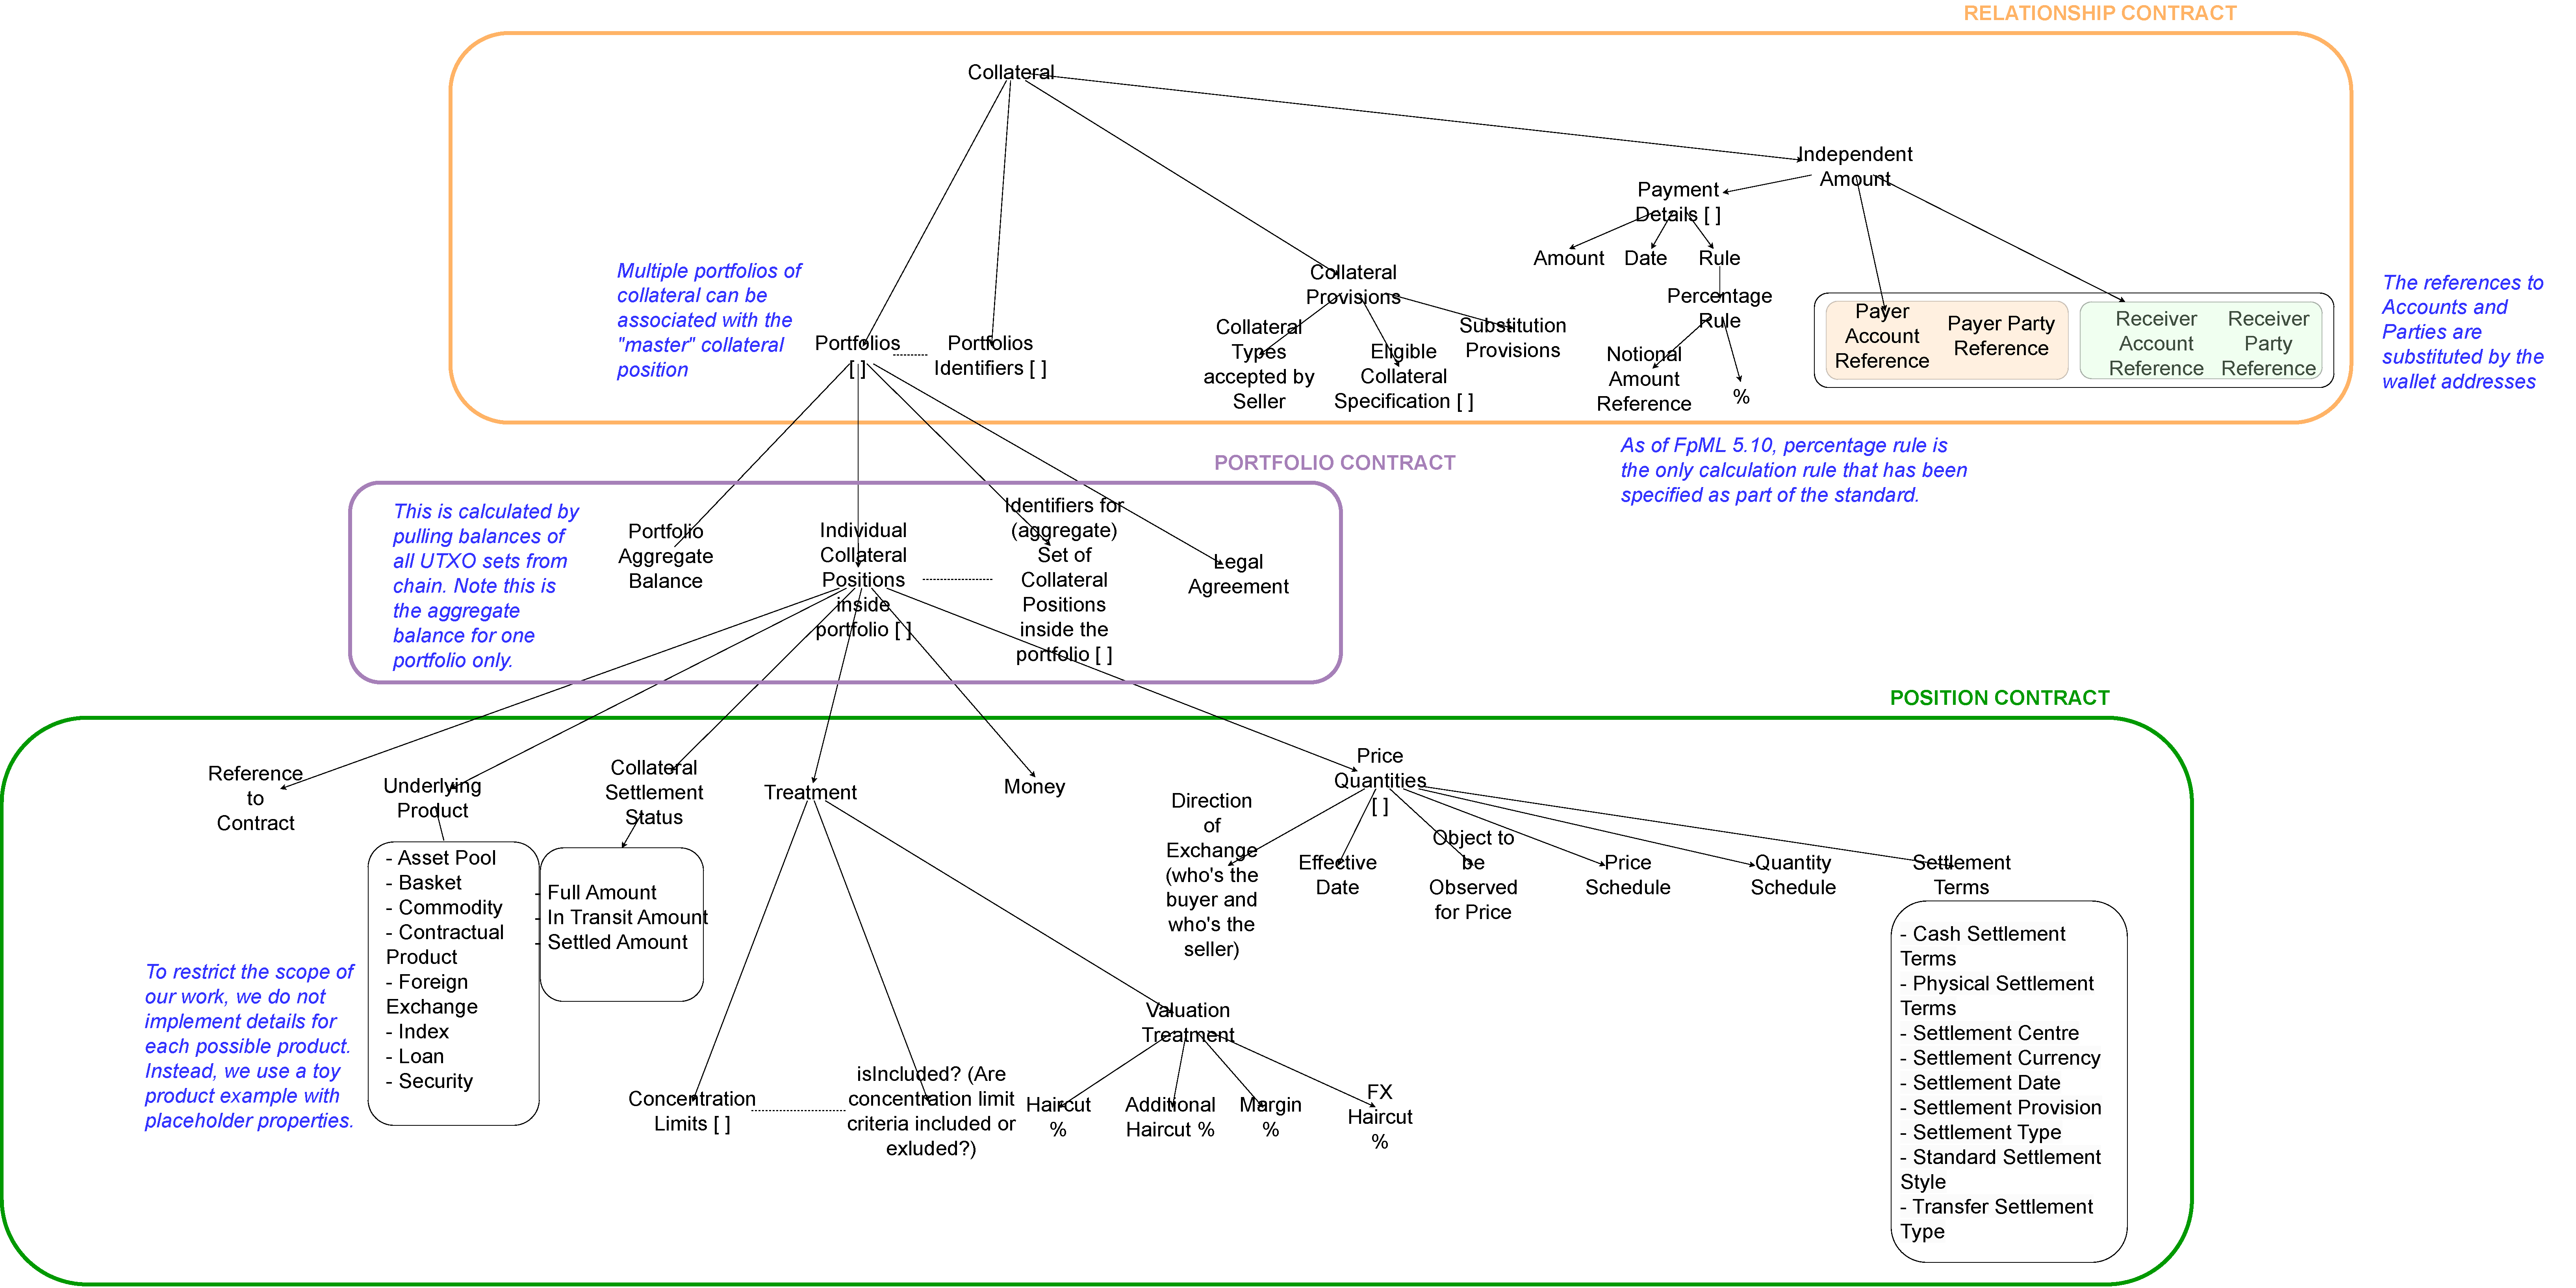
\includegraphics[angle=90, width=0.8\textwidth]{images/chapter 3/mapping (for draft).drawio.pdf}
    \caption[Mapping Common Domain Model to Smart Contracts]{Illustration of the ISDA Common Domain Model (CDM) in a tree-like arrangement. Incoming edges denote containment of one type within another. The CDM is organized into three tiers of smart contracts. The Relationship contract signifies the trading relationship between counterparties, unrelated to specific collateral. The Portfolio contract oversees a group of collateral positions under a shared legal agreement. The Position contract outlines collateral details like type, treatments, and history of movements. }
    \label{fig:mapping}
\end{figure}
\restoregeometry

A key aspect of the dynamics between the different contracts is the ability to reference each other in multiple directions (e.g. fetching individual collateral positions starting from the relationship as well as retrieving the relationship details from any one position). Two approaches have been considered to include this property in our system.

\begin{enumerate}
    \item \label{item:arrays} Our original approach envisioned using arrays to store references to other contracts in the form of UTXO addresses. A challenge was quickly encountered in this scenario due to the fact that sCrypt's array implementations does not allow for variable-sized arrays, only fixed-size \citep{scrypt_arrays}. This would make it impossible to append new portfolios to a relationship or positions to a portfolio. As a workaround to this issue we originally considered storing only references from 'children' contracts to 'parents', removing the \textit{Individual Collateral Position Portfolio} array from a Portfolio and the \textit{Portfolios} array from a Relationship. This way, deploying a new Position, for example, would only require knowing the address of the containing Portfolio at deployment time and include it in the Position, and no arrays would have to be modified. Implementing the bi-directional retrieval capability would have required, however, some complex reverse-indexing \citep{inverted_index} taking place off-chain. This solution appeared cumbersome and complex and was therefore discarded.

    \item We developed an alternative solution, which is the one currently adopted by the system, after support talks with the main sCrypt developers. This solution uses HashedSet to store references to UTXO addresses. An HashedSet \citep{hashed_set} is defined as a special type of HashedMap \citep{hashed_map}, a data structure that efficiently stores key-value pairs by using a hash function to compute indexes for quick retrieval and insertion. A HashedSet is a subtype of a HashedMap where values are identical to their corresponding keys and are thus omitted. A key aspect of the sCrypt implementation of HashedSets is that only the hash values of the keys are saved on the chain, meaning that off-chain copies of the items in the set must be stored locally to be able to deserialize the set into an intelligible representation (hash functions are designed to be one-way functions, making it extremely difficult to retrieve the original input from the hash value \citep{invert_hash_functions}). While adding some technical complexity to the final solution, this approach achieves the bi-directional referencing currently supported by the CDM and we deemed this design to be more feasible and elegant than the original one involving arrays

\end{enumerate}

As already mentioned, mapping the CDM to sCrypt has proven particularly challenging for a number of technical reasons described below:

\begin{itemize}

    \item \textbf{Data types supported by sCrypt}. sCrypt supports three main basic data types, namely \textit{boolean}, \textit{bigint} and and \textit{ByteString}. While the CDM also uses the boolean type, it relies on the \textit{number} and \textit{string} primitives. All references to these two data types had to be converted to \textit{bigint} and \textit{ByeString}, respectively. The rationale behind the choice of these two particular data types to represent numbers and text is not provided in the sCrypt documentation, and while requiring some manual work to convert the CDM, we speculate on the utility of these two data types specifically in a blockchain context:

    \begin{itemize}
        \item \textbf{Bigint} (represents numeric values which are too large to be represented by the number primitive in Typescript \citep{bigint}).
        
        \begin{itemize}
            \item \textbf{Precision}. BSV operates on very large numbers, especially when dealing with satoshis. Regular \textit{numbers} have limited precision, while \textit{BigInt}s can accurately represent and perform arithmetic operations on integers of arbitrary size without loss of precision (and only a 5.30\% performance difference as measured in arithmetic operations per second at the time of writing \citep{bigint_number_performance}).
            \item \textbf{Consistency with Bitcoin Protocol}. The Bitcoin protocol itself uses 64-bit integers for various purposes, therefore BigInt is a better match for representing these integers in a way that aligns with the underlying protocol.
            \item \textbf{Security and Trust}. Using BigInt helps minimize the risk of bugs caused by floating-point inaccuracies and ensures that the code behaves as expected.
        \end{itemize}
        
        \item \textbf{ByteString} (represents arbitrary binary data, ensuring this is handled as raw bytes rather than interpreted characters)

        \begin{itemize}
            \item \textbf{Script operations}. BSV transactions often involve manipulating raw binary data (like public keys, hashes, signatures) rather than traditional text data. Using ByteString can help represent this data more accurately and efficiently.

            \item \textbf{Hexadecimal Representation}. in BSV data is often represented in hexadecimal format (base16). Using a ByteString or binary data representation can make it easier to work with and manipulate these hex-encoded values.

            \item \textbf{Data (De)serialization}. Data serialization and deserialization efficiency\footnote{Efficiency here encompasses both temporal and spatial considerations. Compact data representations are crucial because blockchain memory is a limited resource; using it judiciously minimizes transaction fees. Additionally, quick data operations are imperative for supporting the high throughput of transactions in the financial derivative contexts.} is pivotal due to constraints such as block size limitations. Binary data representation can facilitate more compact serialization formats, thereby optimizing both transaction size and associated fees.

            \item \textbf{Data Integrity}. Using binary data representation can help ensure data integrity by preventing unintended character encoding or transformations that could affect calculations.
            
        \end{itemize}
        
    \end{itemize}

    \item \textbf{Floating point numbers}. While the BigInt datatype ensures higher precision with integer calculations, it does not support floating point calculation, which in our context would be required. For example, the spot price of an asset or the exchange rate between USDC and BSV are all floating point numbers. The current solution truncates the decimal part by taking the floor of the floating point number. Possible workarounds to this barrier are discussed in Section \ref{ch:conclusions}.

    \item \textbf{Dates}. The CDM relies on the built-in Date object in Typescript to represent points in time \citep{dates}. Consistency with this approach would have required translating part of the Typescript implementation itself to utilise the basic sCrypt data types, which we considered out of the scope for this work. A suggested workaround is to simply use a BigInt value that represents the UNIX epoch time (the number of milliseconds since the midnight at the beginning of January 1, 1970, UTC \citep{epoch})

    \item \label{item:generics} \textbf{Generics}. These are reusable and flexible code components in Typescript that allow types to be parameterised, enabling functions, classes, and interfaces to work with different data types while maintaining type safety and preventing the need for code duplication \citep{generics}. For example, the \textit{FieldWithMeta$\langle $T $\rangle$} interface defined in the \textit{metatypes.ts} file of the CDM allows to encapsulate a value of any generic type $T$ along with accompanying metadata within a single structure. Generics are not supported by sCrypt, the compiler yielding an \textit{Invalid Type} error. A possible workaround to to this obstacle would be to create specific variations of the generic interface for all possible types to be supported (sCrypt does support user-defined types \citep{user-defined-types}), effectively violating the very purpose of generics. This has not implemented in the current version of the system as it would have required significant additional manual work that would have not added any major benefits for the purpose of the proof-of-concept and is suggested as future work.

    \item \textbf{Arrays}. As already mentioned on page \pageref{item:arrays}, sCrypt only supports fixed-size arrays. This poses an issue when a type contains arrays that could potentially be empty at deployment and will need to be filled in later. For example, the \textit{EligibleCollateralCriteria} interface contains an array of \textit{IssuerCriteria[]}, specifying requirements or qualifications that an issuer of a financial instrument must meet in order for that instrument to be considered acceptable as collateral, which could be potentially empty at the beginning in case no criteria apply to the type of issuer of the instrument. Assuming the arrays are fixed-size, it makes sense that the compiler would not allow to use empty arrays as these could not be modified while at the same time occupying block size. We originally tried to apply the same workaround described on page \pageref{item:arrays} utilising \textit{HashedSet}s instead of arrays, however the compiler would still throw errors in case the HashedSet was empty at deployment. A possible solution --- not implemented in the system, which currently simply ignores empty arrays --- would be to redeploy a new contract when the values to populate the array are known, ignoring the UTXO corresponding to the previous state.

    \item \label{item:circular_deps} \textbf{Circular dependencies}. In a strongly typed language like TypeScript, a circular dependency between types occurs when two or more types depend on each other directly or indirectly. This can lead to a situation where the types reference each other in a way that creates a loop, making it difficult for the compiler to properly infer and resolve the types \citep{circular_dependencies}. In the CDM, many circular dependencies are present. For example, the \textit{Underlying Product} for the collateral position could be of type \textit{Basket}, which contains multiple \textit{Basket Component}s that could potentially be \textit{Basket}s themselves. Such dependencies would prevent compilation from succeeding, therefore we had to manually amend the types that were generating the problem. While far from optimal, we opted for this workaround as a more thorough solution would have required a deeper overhaul of the CDM itself which was outside the scope of this work. As discussed in \ref{ch:conclusions}, we suggest close collaboration between sCrypt developers and CDM should be fostered to increase the level of interoperability between the two tools.

    
\end{itemize}